\documentclass{article}
\usepackage{tikz}
\usetikzlibrary{positioning}

\begin{document}

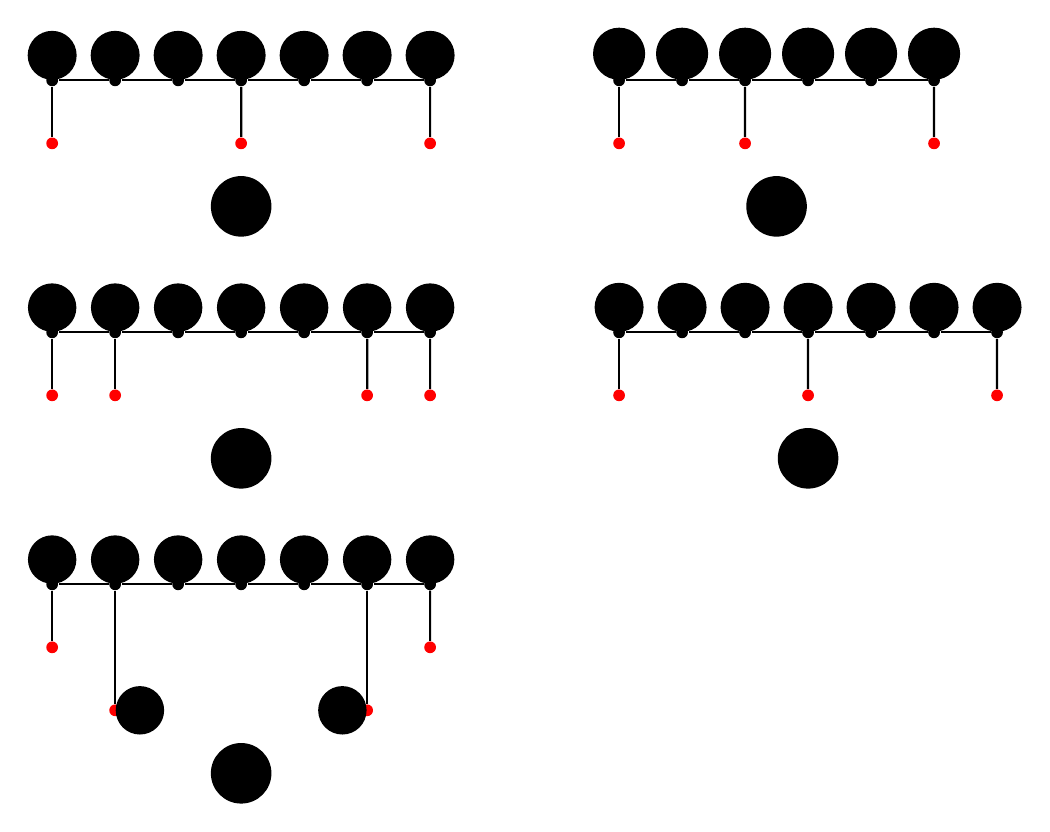
\begin{tikzpicture}[scale=0.8, every node/.style={circle, inner sep=1.5pt, fill=black}]
    % Define styles for red nodes and edges
    \tikzset{
        rednode/.style={fill=red},
        edge/.style={draw, thick}
    }

    % Subfigure (1)
    \begin{scope}[shift={(0,0)}]
        \foreach \x in {0,...,6} {
            \node (\x) at (\x,0) {};
        }
        \foreach \x [count=\xi from 0] in {1,...,6} {
            \draw[edge] (\xi) -- (\x);
        }
        \node[rednode] (r1) at (0,-1) {};
        \node[rednode] (r2) at (3,-1) {};
        \node[rednode] (r3) at (6,-1) {};
        \draw[edge] (0) -- (r1);
        \draw[edge] (3) -- (r2);
        \draw[edge] (6) -- (r3);
        \node at (3,-2) {\textbf{(1)}};
        \node[above] at (0,0) {$S_1$};
        \node[above] at (1,0) {$S_2$};
        \node[above] at (2,0) {$S_3$};
        \node[above] at (3,0) {$S_4$};
        \node[above] at (4,0) {$S_5$};
        \node[above] at (5,0) {$S_6$};
        \node[above] at (6,0) {$S_7$};
    \end{scope}

    % Subfigure (2)
    \begin{scope}[shift={(9,0)}]
        \foreach \x in {0,...,5} {
            \node (\x) at (\x,0) {};
        }
        \foreach \x [count=\xi from 0] in {1,...,5} {
            \draw[edge] (\xi) -- (\x);
        }
        \node[rednode] (r1) at (0,-1) {};
        \node[rednode] (r2) at (2,-1) {};
        \node[rednode] (r3) at (5,-1) {};
        \draw[edge] (0) -- (r1);
        \draw[edge] (2) -- (r2);
        \draw[edge] (5) -- (r3);
        \node at (2.5,-2) {\textbf{(2)}};
        \node[above] at (0,0) {$S'_1$};
        \node[above] at (1,0) {$S'_2$};
        \node[above] at (2,0) {$S'_3$};
        \node[above] at (3,0) {$S'_4$};
        \node[above] at (4,0) {$S'_5$};
        \node[above] at (5,0) {$S'_6$};
    \end{scope}

    % Subfigure (3)
    \begin{scope}[shift={(0,-4)}]
        \foreach \x in {0,...,6} {
            \node (\x) at (\x,0) {};
        }
        \foreach \x [count=\xi from 0] in {1,...,6} {
            \draw[edge] (\xi) -- (\x);
        }
        \node[rednode] (r1) at (0,-1) {};
        \node[rednode] (r2) at (1,-1) {};
        \node[rednode] (r3) at (5,-1) {};
        \node[rednode] (r4) at (6,-1) {};
        \draw[edge] (0) -- (r1);
        \draw[edge] (1) -- (r2);
        \draw[edge] (5) -- (r3);
        \draw[edge] (6) -- (r4);
        \node at (3,-2) {\textbf{(3)}};
        \node[above] at (0,0) {$T_1$};
        \node[above] at (1,0) {$T_2$};
        \node[above] at (2,0) {$T_3$};
        \node[above] at (3,0) {$T_4$};
        \node[above] at (4,0) {$T_5$};
        \node[above] at (5,0) {$T_6$};
        \node[above] at (6,0) {$T_7$};
    \end{scope}

    % Subfigure (4)
    \begin{scope}[shift={(9,-4)}]
        \foreach \x in {0,...,6} {
            \node (\x) at (\x,0) {};
        }
        \foreach \x [count=\xi from 0] in {1,...,6} {
            \draw[edge] (\xi) -- (\x);
        }
        \node[rednode] (r1) at (0,-1) {};
        \node[rednode] (r2) at (3,-1) {};
        \node[rednode] (r3) at (6,-1) {};
        \draw[edge] (0) -- (r1);
        \draw[edge] (3) -- (r2);
        \draw[edge] (6) -- (r3);
        \node at (3,-2) {\textbf{(4)}};
        \node[above] at (0,0) {$S_1$};
        \node[above] at (1,0) {$S_2$};
        \node[above] at (2,0) {$S_3$};
        \node[above] at (3,0) {$S_4$};
        \node[above] at (4,0) {$S_5$};
        \node[above] at (5,0) {$S_6$};
        \node[above] at (6,0) {$S_7$};
    \end{scope}

    % Subfigure (5)
    \begin{scope}[shift={(0,-8)}]
        \foreach \x in {0,...,6} {
            \node (\x) at (\x,0) {};
        }
        \foreach \x [count=\xi from 0] in {1,...,6} {
            \draw[edge] (\xi) -- (\x);
        }
        \node[rednode] (r1) at (0,-1) {};
        \node[rednode] (r2) at (1,-2) {};
        \node[rednode] (r3) at (5,-2) {};
        \node[rednode] (r4) at (6,-1) {};
        \draw[edge] (0) -- (r1);
        \draw[edge] (1) -- (r2);
        \draw[edge] (5) -- (r3);
        \draw[edge] (6) -- (r4);
        \node at (3,-3) {\textbf{(5)}};
        \node[above] at (0,0) {$T_1$};
        \node[above] at (1,0) {$T_2$};
        \node[above] at (2,0) {$T_3$};
        \node[above] at (3,0) {$T_4$};
        \node[above] at (4,0) {$T_5$};
        \node[above] at (5,0) {$T_6$};
        \node[above] at (6,0) {$T_7$};
        \node[right] at (r2) {$T_2$};
        \node[left] at (r3) {$T_5$};
    \end{scope}
\end{tikzpicture}

\end{document}